\section{Основные понятия}

В прошлой главе мы уже упоминали вскользь множества, сейчас же займемся ими более плотно. Вспомним во-первых то что уже определяли ранее:

{\bfseries Определение.} {\slshape Множеством} называется неупорядоченный набор различимых объектов, называемых {\slshape элементами} множества.

Это определение на самом деле не слишком строгое, и при желании из него можно вывести всякие парадоксальные и противоречивые следствия, ввиду чего математиками принято более строгое аксиоматическое задание множеств. В большинстве случаев, однако, такое определение вполне достаточно, и оно является куда более интуитивным и наглядным, нежели строгое определение, поэтому вначале мы будем работать с ним, а под конец главы я уже дам строгую аксиоматизацию теории множеств, когда какая-то интуиция о них уже будет иметься.

Задать множества можно многими способами, самый простой из которых заключается в простом перечислении элементов множества. Например, множество всех гласных английского алфавита можно записать как $V = \{a, e, i, o, u\}$. Можно было бы впрочем описать его и просто словами: «$V$ — это множество гласных английского алфавита». Суть от этого не поменялась бы.

Обратим внимание на слова «неупорядоченный» и «различимые». Неупорядоченность означает, что $\{a, e, i, o, u\} = \{u, o, a, e, i\}$, то есть нам не важно в каком порядке множество задано, важен лишь его состав. «Различимость» говорит о том, что набор элементов $\{a, a, e, e, i\}$ множеством в математическом смысле уже не является — множество не может по определению содержать совершенно одинаковые объекты, которые мы не можем различить.

В первой главе мы уже сталкивались со многими понятиями, которые являются множествами (могут рассматриваться как множества), и которые могут быть хорошими примерами: множество логических значений $\{0, 1\}$, множество всех формул, множество моделей заданной теории $\mathrm{Mod}(T)$, множество логических функций, и так далее. Из более приземленных примеров можно рассматривать множество всех звезд на небе, множество учащихся младших классов, множество монет у меня в кармане и подобные.

Отдельного упоминания заслуживает следующее тривиальное, но очень важное множество:

{\bfseries Определение.} Множество $\emptyset=\{\}$, не содержащее ни одного элемента, называется {\slshape пустым множеством}.

Если $x$ является элементом множества $S$, то это обозначается как $x \in S$. Если не является, то это обозначается как $x \not\in S$.

Пустое множество таким образом можно охарактеризовать следующим логическим утверждением: $\forall x, x \not \in \emptyset$.

Второе определение, которое было в первой главе, это определение подмножества:

{\bfseries Определение.} Множество $A$ называется {\slshape подмножеством} множества $B$ (обозначение $A\subset B$), если любой элемент из $A$ содержится так же и в множестве $B$.

На языке логики это определение можно записать так: $\forall x, (x\in A\rightarrow x\in B)$.

Очевидно следующее простое свойство: $\forall X, \emptyset\subset X$, то есть пустое множество является подмножеством любого другого множества. Это может быть непонятно исходя из интуитивного словесного определения, но идеально вписывается в приведенную логическую формулу для подмножеств: высказывание $x\in\emptyset$ всегда ложно, следовательно, импликация $x\in\emptyset \rightarrow X$, всегда истинна, чем бы не являлось $X$. Это демонстрирует преимущество строгих логических формулировок над интуитивными определениями: определение на языке логики всегда позволяет однозначно ответить на ряд вопросов, которые в противном случае могут даже не иметь смысла. По этой причине (а так же в качестве упражнения для мозга) последующие определения мы будем давать сразу сразу и на языке логики, и на обычном человеческом языке.

Так же полезно вспомнить, что каждое подмножество может быть задано некоторым предикатом, и по каждому подмножеству можно построить предикат. Множества, заданные предикатами, записываются так: $\{x \in A|P(x)\}$ — так описывается подмножество множества $A$, для элементов которых оказывается истинным предикат $P$.

{\bfseries Определение.} Множества $A$ и $B$ называются равными ($A=B$), если они состоят из одних и тех же элементов: $\forall x, (x\in A \leftrightarrow x\in B)$.

Кто читал первую главу, знает, что $(x\in A \leftrightarrow x\in B) = (x \in A \rightarrow x \in B) \wedge (x \in B \rightarrow x \in A)$, поэтому можно сформулировать следующее свойство:

{\bfseries Теорема.}  $A=B$ тогда и только тогда, когда $A\subset B$ и $B \subset A$.

{\bfseries Определение.} Объединением множеств $A$ и $B$ ($A\cup B$) называется множество, которое содержит элементы обоих множеств: $\forall x, (x\in A \vee x \in B \leftrightarrow x\in A\cup B)$.

Понятно, что если какие-то элементы входят одновременно и во множество $A$ и во множество $B$, то в объединение множеств они войдут лишь в единственном экземпляре:

{\bfseries Пример.} Пусть $A = \{a, b, c, d\}$ и $B = \{b, c, d, e, f\}$. Тогда $A\cup B = \{a, b, c, d, e, f\}$

Логические операции удобно наглядно изображать с помощью так называемых кругов Эйлера. Пример, который я только что привел, может быть графически изображен следующим образом:

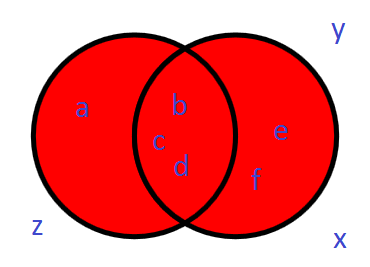
\includegraphics{sets-union.png}
\begin{figure}
\centering
\def\seta{(-1,0) circle (2)}
\def\setb{(1,0) circle (2)}
\begin{tikzpicture}
     \tikzstyle{element}=[minimum size=1mm, font=\large]
    \draw [fill=red]   \seta;
    \draw [fill=yellow]\setb;
    \begin{scope}[even odd rule]
        \clip \seta;
        \fill[fill=orange] \setb;
    \end{scope}
    \draw \seta;
    \draw \setb;
    \foreach \t/\x/\y in { z/-3/-2, x/3/-2, y/3/2, a/-2/0, b/-.1/1, c/.3/0, d/-.2/-1,
    e/2/.5, f/1.5/-.5 }
        \node[element] (\t) at (\x,\y) {$\t$};
\end{tikzpicture}
\caption{Пересечение двух множеств}
\end{figure}


Здесь $x$, $y$ и $z$ — это просто некоторые элементы, которые не вошли ни в одно из множеств. Всегда при работе со множествами (да и вообще всегда) важно рассматривать не только объекты, с которыми мы непосредственно работаем, но и внешние факторы. Красным цветом обозначено объединение двух множеств, представляемых кругами.

{\bfseries Определение.} Пересечением множеств $A$ и $B$ ($A\cap B$) называется множество, которое содержит лишь те элементы которые принадлежат сразу обоим множествам: $\forall x, (x\in A \wedge x \in B \leftrightarrow x\in A\cap B)$.

{\bfseries Пример.} Пусть $A = \{a, b, c, d\}$ и $B = \{b, c, d, e, f\}$. Тогда $A\cap B = \{b, c, d\}$

{\bfseries Упражнение.} Нарисуйте круги Эйлера для пересечения множеств (какую часть рисунка надо закрасить цветом?)

{\bfseries Определение.} Множества называются {\slshape непересекающимися}, если $A\cap B = \emptyset$ (то есть множества не имеют общих элементов). В противном случае множества называются пересекающимися.

{\bfseries Пример.} Множества $\{a, b, c\}$ и $\{d, e, f\}$ не пересекаются. Множества $\{a, b\}$ и $\{b, c\}$ пересекаются, и их пересечением является множество $\{b\}$.

{\bfseries Определение.} Разностью множеств $A\setminus B$ называется множество, содержащее все те элементы $A$, которые не содержатся в $B$: $\forall x, (x \in A\cap B \leftrightarrow x\in A \wedge x \not \in B)$.

{\bfseries Пример.} Пусть $A = \{a, b, c, d\}$ и $B = \{b, c, d, e, f\}$. Тогда $A\setminus B = \{a\}$

{\bfseries Упражнение.} Нарисуйте круги Эйлера для разности множеств.

{\bfseries Определение.} {\slshape Симметрической разностью} множеств $A\bigtriangleup B$ называется множество $(A\setminus B)\cup (B\setminus A)$, то есть множество элементов, принадлежащих либо $A$, либо $B$, но не их пересечению: $\forall x,(x\in A\bigtriangleup B \leftrightarrow x\in A \oplus x\in B)$.

{\bfseries Пример.} Пусть $A = \{a, b, c, d\}$ и $B = \{b, c, d, e, f\}$. Тогда $A\bigtriangleup B = \{a, e, f\}$.

{\bfseries Упражнение.} Нарисуйте круги Эйлера для симметрической разности множеств.

Часто при работе со множествами, мы держим в уме, что все элементы нашего множества являются элементами некоторого другого более крупного множества, содержащего все возможные объекты рассматриваемой нами задачи. Например, если мы говорим о множестве звёзд на небе, то мы можем держать в уме так же множество всех звезд вообще, а не только видимых нам. Если мы говорим о множестве учеников десятого класса школы N469, то как более общее множество мы можем подразумевать множество вообще всех учеников этой школы, либо же множество всех школьников страны, либо же множество всех людей. Смотря что за задачу мы решаем. Поэтому оказывается полезным ввести следующее определение:

{\bfseries Определение.} {\slshape Универсальным множеством}, или {\slshape универсумом}, называется множество всех возможных элементов, имеющих смысл в решаемой задаче.

{\bfseries Пример.} Если посмотреть на круги Эйлера, приведенные выше для иллюстрации объединения множеств и считать, что на картинке представлены все интересные нам элементы, то там универсумом в этом случае является множество $U = \{a, b, c, d, e, f, x, y, z\}$.

{\bfseries Определение.} {\slshape Дополнением} множества $A$ (обозначается как $A^C$) называется множество элементов универсума, не принадлежащих множеству $A$: $\forall x, x\in A^C \leftrightarrow x\in U \wedge x \not \in A$, где $U$ — универсум. Это же можно записать и без упоминания универсума, если предположить, что мы держим его «в уме»: $\forall x, x\in A^C \leftrightarrow x\not \in A$.

Понятно, что для операции дополнения необходимо строгое задание универсума, иначе она теряет смысл.

{\bfseries Пример.} Пусть $U = \{a, b, c, d, e, f, x, y, z\}$ и $A = \{a, b, c, d\}$. Тогда $A^C = \{e, f, x, y, z\}$.

{\bfseries Упражнение.} Нарисуйте круги Эйлера для дополнения.

Основные понятия мы определили, теперь надо разобраться с их свойствами. Однако прежде чем мы сформулируем нашу первую теорему о множествах, сделаем такое существенное наблюдение: практически все логические операции и операции над множествами находятся в соответствии друг с другом и операции над множествами определяются просто через логические операции. Так, логическое И задает пересечение множеств. Логическое ИЛИ — объединение. Исключающее ИЛИ — симметрическую разность. Отрицание высказываний — дополнение множеств. Эквиваленция — равенство множеств. Импликация — подмножества. В некотором смысле можно так же провести аналогию между универсумом и истинным высказыванием, а так же пустым множеством и ложным высказыванием.

Для продвинутых читателей, которые целиком осилили и поняли первую главу, отмечу, что сильно извратившись (как раз как я люблю), определить можно не только операции над множествами через операции над высказываниями, но и наоборот. Пусть, например, у нас есть теория $T_0$ и формулы $\phi$ и $\psi$. Пусть у нас так же есть теория $T_1$, для которой известно, что $\mathrm{Mod}(T_1) = \mathrm{Mod}(T_0, \phi) \cup \mathrm{Mod}(T_0, \psi)$. Тогда можно показать (сделайте это самостоятельно), что теория $T_1 = T_0 \cup \{\phi\vee \psi\}$ будет иметь как раз требуемое множество моделей (хотя такая теория может быть конечно не единственна), и именно через свойства моделей при добавлении формул можно определить логическое ИЛИ. Нечто аналогичное мы делали, когда определяли понятие импликации. Нечто аналогичное можно сделать и для всех других логических операций.

{\bfseries Теорема 1}. Для операций над множествами справедливы следующие законы:

{\slshape Ассоциативность:}

1) $(A \cap B) \cap C = A \cap (B \cap C)$

2) $(A \cup B) \cup C = A \cup (B \cup C)$

3) $(A \bigtriangleup B) \bigtriangleup C = A \bigtriangleup (B \bigtriangleup C)$

{\slshape Коммутативность:}

4) $A \cap B = B \cap A$

5) $A \cup B = B \cup A$

6) $A \bigtriangleup B = B \bigtriangleup A$

7) $A = B$ равносильно $B = A$.

{\slshape Дистрибутивность:}

8) $A \cap (B \cup C) = (A \cap B) \cup (A \cap C)$

9) $A \cup (B \cap C) = (A \cup B) \cap (A \cup C)$

10) $A \cap (B \bigtriangleup C) = (A \cap B) \bigtriangleup (A \cap C)$

{\slshape Двойное дополнение:}

11) $(A^C)^C = A$

{\slshape Законы де Моргана:}

12) $(A \cap B)^C = A^C \cup B^C$

13) $(A \cup B)^C =A^C \cap B^C$

{\slshape Еще по мелочам (здесь $U$ — универсальное множество):}

14) $A \cap U = A$

15) $A \cap \emptyset = \emptyset$

16) $A \cup U = U$

17) $A \cup \emptyset = A$

18) $A \bigtriangleup \emptyset = A$

19) $A \bigtriangleup U = A^C$

20) $A \cap A^C = \emptyset$

21) $A \cup A^C = U$

22) $A \bigtriangleup A^C = U$

23) $A\cap A = A$

24) $A\cup A = A$

25) $A \bigtriangleup A = \emptyset$

26) $A \cap (A^C \cup B) = A \cap B$

27) $A \cup (A^C \cap B) = A \cup B$

{\slshape Новенькое для отрицания:}

28) $A \setminus B = A \cap B^C$

{\slshape Свойства подмножеств:}

29) Если $A \not \subset B$, то $A$ и $B^C$ пересекаются.

30) $A \subset A$

31) Транзитивность: $A \subset B \wedge B \subset C \rightarrow A \subset C$ (думаю на всякий случай это свойство полезно проговорить словами: если $A\subset B$ и $B\subset C$, то $A\subset C$)

32) $A \subset B\cap C \rightarrow A \subset B$

33) Если $A \subset B$, то $B^C \subset A^C$ и наоборот.

{\bfseries Доказательство.} Во-первых, как можно заметить, все эти свойства дублируют соответствующие свойства для логических операций. Такой вот поворот событий. Некоторые свойства пришлось немного переформулировать (в основном в части с импликацией), одно свойство добавилось для разности множеств, несколько свойств потеряли смысл в теории множеств либо стали неинтересны. Но в целом мы имеем то же самое один в один.

Доказательства всех этих свойств оказываются совершенно элементарны и сводятся, как можно догадаться, к простой переформулировке на языке логики. Давайте докажем, например свойство 10 (мы здесь активно используем задание подмножеств предикатами, которые в нашем случае являются простой логической формулой, а так же дистрибутивность из теоремы 1 главы 1):

$A \cap (B \bigtriangleup C) = \{x|x\in A \wedge x \in B\bigtriangleup C\} = \{x|x\in A \wedge (x \in B \oplus x \in C)\}\\ = \{x|(x\in A \wedge x \in B) \oplus (x \in A \wedge x \in C)\} = \{x|(x\in A \cap B) \oplus (x \in A \cap C)\} \\ = \{x|x\in (A \cap B) \bigtriangleup (A \cap C)\} = (A \cap B) \bigtriangleup (A \cap C)$

Что и требовалось. Как видно из этих рассуждений, операции над множествами и операции над высказываниями — это действительно очень близкие понятия, которые во многом отражают одно и то же, только несколько под разным углом.

Остальные свойства докажите самостоятельно в качестве упражнения, а так же нарисуйте круги Эйлера для этих свойств — они должны дать довольно не плохую интуицию относительно свойств множеств (и заодно логики). \qed

В завершение параграфа определим еще одну операцию, которая уже не имеет никакого прообраза в логике.

{\bfseries Определение.} {\slshape Булеаном} множества $A$ (обозначается $2^A$) называется множество всех его подмножеств.

{\bfseries Пример.} Пусть $A = \{a, b, c\}$. Тогда $2^A = \{\emptyset, \{a\}, \{b\}, \{c\}, \{a, b\}, \{a, c\}, \{b, c\}, A\}$.

Обратите внимание, что всегда $\emptyset \in 2^A$ и $A\in 2^A$. Так же обратите внимание на то, что булеан, сам являясь множеством, содержит в качестве своих элементов другие множества (это ничему не противоречит — элементами множеств могут быть и другие множества, почему бы и нет?).

Так же важно отметить такой нюанс: если $a \in A$, то $\{a\} \in 2^A$, но $a \not \in 2^A$. Это довольно очевидно: $a\not = \{a\}$, ведь множество состоящее из одного элемента и сам этот элемент логически разные сущности.

Понятие булеана будет активно использоваться нами в дальнейшем, а пока мы рассмотрим опять же аналогию булеана с логикой (это только для дотошных читателей). Пусть $A$ — некоторое одноэлементное множество. Тогда $2^A = \{\emptyset, A\}$.Теперь, если рассматривать наши операции над множествами, ограничившись лишь этим булеаном, то если назвать $\emptyset$ ложью, а $A$ истиной, то наша аналогия между логическими операциями и операциями над множествами станет уже не примерной, а совершенно однозначной.

Таким образом можно считать, что логика — это в некотором смысле частный случай теории множеств, которая в свою очередь является обобщением логики. Если рассматривать $A$, который состоит из многих элементов, то можно в некотором смысле говорить, что $2^A$ — это модель нечеткой логики, где $A$ — истинное высказывание, $\emptyset$ — ложное высказывание, а остальные множества являются истинными высказываниями лишь с некоторой степенью вероятности. Это далеко не самый удобный подход для определения нечеткой логики, и на практике математиками не используется наверное никогда, кроме очень узких областей, однако мы будем иногда обращаться к этому примеру в качестве иллюстраций и более интуитивного понимания отдельных понятий.

Так же у дотошного читателя может возникнуть определенный дискомфорт от той последовательности изложения, которую он до сих пор наблюдает: говоря о логике и предикатах мы ввели понятие множеств, говоря о множествах мы во всю опирались на логигу. Это как в России: чтобы получить работу по специальности, надо иметь опыт работы по этой специальности, а чтобы получить опыт, надо проработать по этой специальности. Такие ситуации допустимы в быту, но не в науке, поэтому порочные круги необходимо разрывать.

Пока я стараюсь дать просто интуицию о множествах, поскольку строгое формальное изложение без порочных кругов и без начальной интуиции вряд ли окажется сильно полезно и понятно читателю. Поэтому пока мы оставим все как есть, а формальное изложение проведем в конце главы, где уже окончательно расставим все на свои места и избавимся от всех неточностей и нечеткости в определениях.
